\chapter{Mathematical Circuits Using Op.Amp.: Part II}


\section{Objectives}
\begin{itemize}
    \item To verify Op.Amp. circuits for differentiation operation
    \item To verify Op.Amp. circuits for integration operation
    \item To verify Op.Amp. circuits for logarithm operation
    \item To verify Op.Amp. circuits for exponentiation operation
\end{itemize}

\section{Materials}
\begin{itemize}
    \item Breadboard
    \item Capacitors
    \item DC power supply
    \item Digital Multi-Meter
    \item \hyperref[1N4148]{Diode (1N4148)}
    \item Function Generator
    \item \hyperref[LM741_1]{Op.Amp. (LM741)}
    \item Oscilloscope
    \item Resistors
\end{itemize}

\section{Introduction}
    \subsection{Circuit Diagram}
    \begin{figure}[h]

        \begin{subfigure}[h]{0.47\textwidth}
        \begin{center}
            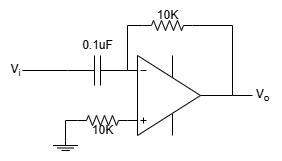
\includegraphics[width=1\linewidth]{Lab11/Lab11a.drawio.png}
            \caption{}
            \label{L11a}
        \end{center} 
        \end{subfigure}
    \hfill
    \vspace{0.2 cm}
        \begin{subfigure}[h]{0.47\textwidth}
        \begin{center}
            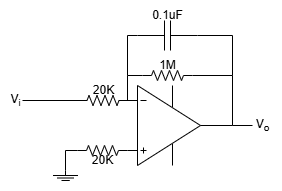
\includegraphics[width=1\linewidth]{Lab11/Lab11b.drawio.png}
            \caption{}
            \label{L11b}
        \end{center}
        \end{subfigure}
    \vfill
    
    \vspace{0.2 cm}
        \begin{subfigure}[h]{0.47\textwidth}
        \begin{center}
            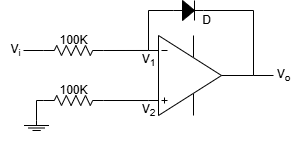
\includegraphics[width=1\linewidth]{Lab11/Lab11c.drawio.png} 
            \caption{}
            \label{L11c}
        \end{center}
        \end{subfigure}
    \hfill
        \begin{subfigure}[h]{0.47\textwidth}
        \begin{center}
            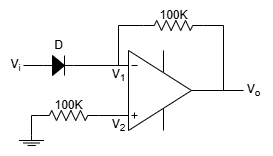
\includegraphics[width=1\linewidth]{Lab11/Lab11d.drawio.png}
            \caption{}
            \label{L11d}
        \end{center}
        \end{subfigure}

    \caption{Different fundamental Op.Amp. circuits}
    \label{l11fs}
    
    \end{figure}
    \FloatBarrier

\section{Detailed Procedures}
    \subsection{Analyzation}


    \subsection{Procedures}

    
\section{Discussion}


\section{Conclusion}
